\begin{Definition}{
	Ist $f: I \rightarrow \mathbb{R}$ beliebig oft differenzierbar, so definieren 
	wir die Taylorreihe am Entwicklungspunkt $\alpha \in I$.
	\begin{align*}
		T_{f, \alpha} (x) = \sum_{n = 0}^{\infty} \frac{f^{(n)}(\alpha)}{n!}
		(x- \alpha)^n
	\end{align*}
	\textbf{Bemerkung:} 
	\begin{itemize}
		\item im Allgemeinen konvergiert $T_{f,\alpha}(x)$ für $x \neq \alpha$ nicht
		\item Der Satz von Taylor behandelt \underline{nicht} die Taylorreihe
		\item Selbst wenn $T_{f, \alpha}(x)$ konvergiert, muss 
		$T_{f,\alpha}(x) = f(x)$ nicht gelten
		\item Sei $R_n(x) = P_{n, \alpha}(x) -f(x)$ Dann gilt :
		\begin{align*}
			P_{n,\alpha}(x) \xlongrightarrow{n \rightarrow \infty} f(x) 
			& \Leftrightarrow  R_n (x) \rightarrow 0
		\end{align*}
	\end{itemize}
}\end{Definition}

\begin{Satz}{
	Sei $f(x) = \sum_{n_0}^{\infty} a_n (x- \alpha)^n $ und $R > 0$ der zugehörige 
	Konvergenzradius von $f$.\\
	Dann ist $f$ auf $(\alpha -R, \alpha + R)$ beliebig oft differenzierbar und 
	es gilt:
	\begin{align*}
		f^{(l)}(\alpha) = l ! \cdot a_l
	\end{align*}
	das heißt, die Taylorreihe $T_{f,\alpha}$ stimmt mit der definierten 
	Potenzreihe überein.
	\\
	\textbf{Beweis:} Wir wissen bereits, dass Potenzreihen gliedweise differenziert
	 werden. Daher gilt: 
	 \begin{align*}
	 	f'(x) = & \left( \sum_{n = 0}^{\infty} a_n (x- \alpha)^n \right) '
	 	 =  \sum_{n= 1}^{\infty}n \cdot a_n (x- \alpha)^{n-1} \\
	 	\vdots \\
	 	f^{(l)} = & l! \cdot a_l + \sum_{n = l-1}^{\infty} n \cdot (n-1) \cdot 
	 	... \cdot (n-l) a_n(x-\alpha)^{n-l}
	 \end{align*}
	 für $l \in \mathbb{N}$ \\
	 \textit{$(x - \alpha) = 0$ für $x = \alpha$}\\
	 Also: $f^{(l)}(\alpha) = l! \cdot a_l$
}\end{Satz}

\section{Riemann-Integral}\label{kap_riemann_integral}
\underline{\textbf{Ziel}:} Wir wollen auf \enquote{natürliche}\todo{eigentlich wäre "\\emph" sogar besser als Anführungsstriche} Weise einen 
Flächeninhaltsbegriff definieren, der uns erlaubt, die Fläche zwischen den Graphen 
einer Funktion und der $x-$Achse zu bestimmen (Abbildung~\ref{fig_int_vorgehen}).
	\begin{figure}[ht]
	\begin{center}
		\tikzsetnextfilename{plot_integral_f}

		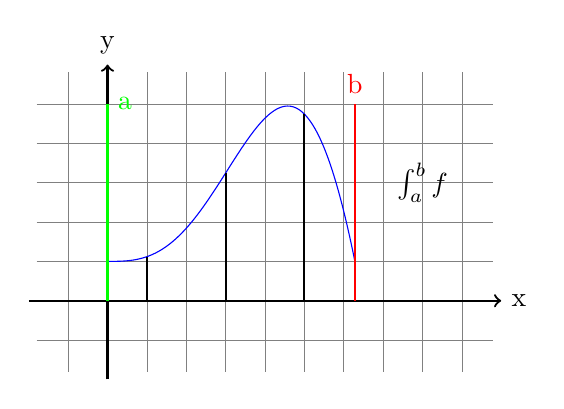
\begin{tikzpicture}
			\draw[very thin, gray, step = 0.5] (-0.9,-0.9) grid (4.9,2.9);
			\draw[->,thick, black](-1,0) -- (5,0) node[right]{x};
			\draw[->,thick, black](0,-1) -- (0,3) node[above]{y};
			\draw[blue,domain = 0.0:3.14, samples=1000]   
				plot (\x,{(\x * \x)*sin(\x r)*0.5+0.5});
	       	\draw[green,thick](0.0,0)--(0.0,2.5)node[right]{a};
	       	\draw[red,thick](3.14,0) -- (3.14,2.5) node[above]{b};
	       	\draw[black,thick](0.5,0) -- (0.5, 0.56);
	       	\draw[black,thick](1.5,0) -- (1.5, 1.62);
	       	\draw[black,thick](2.5,0) -- (2.5, 2.37);
	       	\node at (4,1.5){$\int_a^b f$};
		\end{tikzpicture}
	\end{center}
	\caption{Vorgehen}
	\label{fig_int_vorgehen}
\end{figure}
	
Dabei heißt auf \enquote{natürliche Weise} insbesondere: 
\begin{itemize}
	\item gilt $f(x) = c = const$ für alle $x \in D (f) = [a,b]$, so soll 
	gelten (Abbildung~\ref{fig_int_konst_funk})
	\begin{align*}
		\int_a^b f \dd{x} = c \cdot ( b - a)
	\end{align*}
	\begin{figure}[ht]
	\begin{center}
		\tikzsetnextfilename{plot_rechteck_integral}
		\begin{tikzpicture}
			\draw[dotted, very thin, gray, step = 0.5] (-0.9,-0.9) grid (4.9,2.9);
			\draw[->,thick, black](-1,0) -- (5,0) node[right]{x};
			\draw[->,thick, black](0,-1) -- (0,3) node[above]{y};
			\draw[thick,blue](0,2) -- (4,2) node[right=0.05,fill=white, inner sep=1pt]{f};
			\draw[pattern=north west lines, pattern color=magenta](1,0) rectangle (3.5,2);
			\node[below=0.05, fill=white,inner sep=1pt] at (1,0) {a};
			\node[below=0.05, fill=white,inner sep=1pt] at (3.5,0) {b};
			\node[left=0.05, fill=white,inner sep=1pt] at (0,2) {c};
		\end{tikzpicture}
		\caption{Konstante Funktion}
		\label{fig_int_konst_funk}
	\end{center}
\end{figure}
	
	\item gilt $f(x) \leq g(x)$ $(x \in [a,b])$ so fordern wir (Abbildung~
	\ref{plot_flaeche_zweier_fkt})
	\begin{align*}
		\int_a^b f \dd{x} \leq \int_a^b g(x) \dd{x} 
	\end{align*}
	\begin{figure}[ht]
		\begin{center}
			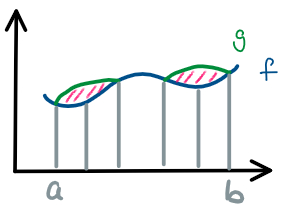
\includegraphics[scale=0.5]{Skizzen/plot_integral_zwei_fkt}
		\end{center}
		\caption{Flächeninhalt zweier Funktionen}
		\label{plot_flaeche_zweier_fkt}
	\end{figure}
	
	\item für $c \in [a,b]$ soll gelten (Abbildung~\ref{fig_integral_aufteilen})
	\begin{align*}
		\int_a^b f \dd{x} = \int_a^c f \dd{x} + \int_c^b f\dd{x}
	\end{align*}
	Vorgehen: Man unterteile $[a,b]$ in \enquote{viele} Teilintervalle, auf denen 
	$f$ nahezu konstant ist.
	\begin{figure}[ht]
\centering
	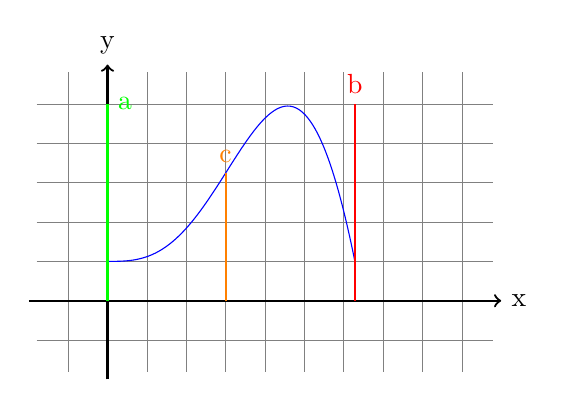
\begin{tikzpicture}
		\draw[very thin, gray, step = 0.5] (-0.9,-0.9) grid (4.9,2.9);
		\draw[->,thick, black](-1,0) -- (5,0) node[right]{x};
		\draw[->,thick, black](0,-1) -- (0,3) node[above]{y};
		\draw[blue,domain = 0.0:3.14, samples=1000]   
			plot (\x,{(\x * \x)*sin(\x r)*0.5+0.5});
       	\draw[green,thick](0.0,0)--(0.0,2.5)node[right]{a};
       	\draw[red,thick](3.14,0) -- (3.14,2.5) node[above]{b};
       	\draw[orange,thick](1.5,0) -- (1.5, 1.62) node[above]{c};
	\end{tikzpicture}
	\caption{Integral aufteilen}
	\label{fig_integral_aufteilen}
\end{figure}
\end{itemize} 

\begin{Definition}{
	Sei $ I \subseteq \mathbb{R}$ ein Intervall. Eine \underline{Partition}\todo{das geht besser auch mit Stichwortverzeichnis. Baue ich später ein.} $P$ 
	(Abbildung~\ref{fig_int_partition}) von 
	$[a,b]$ ist eine endliche Menge von Punkten $a = x_0 \leq x_1 \leq \hdots
	\leq x_n = b$.\\
	Wir schreiben $\Delta x_i = x_i - x_{i-1}$
	\begin{figure}[ht]
       \tikzsetnextfilename{plot_integral_partition}
       \begin{center}
              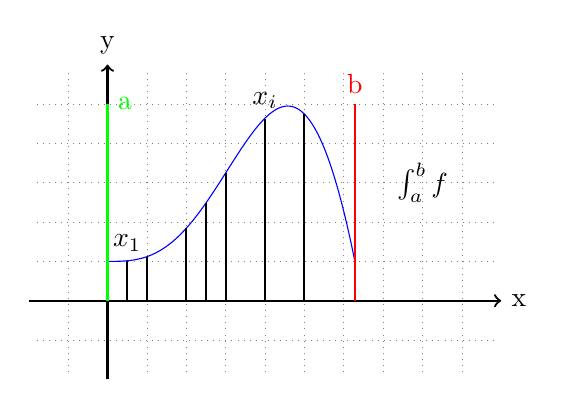
\begin{tikzpicture}
       		\draw[dotted, very thin, gray, step = 0.5] (-0.9,-0.9) grid (4.9,2.9);
       		\draw[->,thick, black](-1,0) -- (5,0) node[right]{x};
       		\draw[->,thick, black](0,-1) -- (0,3) node[above]{y};
       		\draw[blue,domain = 0.0:3.14, samples=1000]   
       			plot (\x,{(\x * \x)*sin(\x r)*0.5+0.5});
              	\draw[green,thick](0.0,0)--(0.0,2.5)node[right]{a};
              	\draw[red,thick](3.14,0) -- (3.14,2.5) node[above]{b};
              	\draw[black,thick](0.25,0) -- (0.25, 0.5)node[above]{$x_1$};
              	\draw[black,thick](0.5,0) -- (0.5, 0.55);
              	\draw[black,thick](1,0) -- (1, 0.92);
              	\draw[black,thick](1.25,0) -- (1.25, 1.24);
              	\draw[black,thick](1.5,0) -- (1.5, 1.62);
              	\draw[black, thick](2,0) -- (2, 2.31) node[above]{$x_i$};
              	\draw[black,thick](2.5,0) -- (2.5, 2.37);
              	\node at (4,1.5){$\int_a^b f$};
       	\end{tikzpicture}
       \end{center}
	\caption{Partition}
	\label{fig_int_partition}
\end{figure}
}\end{Definition}

\begin{Definition}{ \label{def_riemann-integrierbar}
	Sei $f : [a,b] \rightarrow \mathbb{R}$ beschränkt und $P = \{x_0, \hdots, x_n\}$ 
	eine Partition von $[a,b]$.\\
	Wir schreiben: 
	\begin{align*}
		M_i(P) := \sup_{x \in [x_{i-1}, x_i]} f(x) \\
		m_i(p) := \inf_{x \in [x_{i-1}, x_i]} f(x)
	\end{align*}
	Weiter definieren wir: 
	\begin{align*}
		S(P,f) := & \sum_{i=1}^n M_i \cdot \Delta x_i \\
		s(P,f) := & \sum_{i=1}^n m_i \cdot \Delta x_i
	\end{align*}
	Wir setzen:
	\begin{align*}
		\overline{\int_a^b} f \dd{x} = \inf S(P,f) \\
		\underline{\int_a^b} f \dd{x} = \sup s(P,f)
	\end{align*}
	wobei Infimum und Supremum über alle Partitionen von $[a,b]$ genommen werden. 
	Wir nennen 
	\begin{align*}
		& \overline{\int_a^b} f \dd{x} \text{ das \underline{obere} und} \\
		& \underline{\int_a^b} f \dd{x} \text{ das \underline{untere}}
	\end{align*}
	\underline{Riemannintegral} von $f$ über $[a,b]$ \\
	Gilt 
	\begin{align*}
		\int_a^{\overline{b}} f \dd{x} = \int_{\underline{a}}^b f \dd{x}
	\end{align*}
	sagen wir $f$ ist \underline{Riemann-integrierbar} (\underline{integrierbar}) 
	und nennen 
	\begin{align*}
		\int_a^b f(x) \dd{x} := \underline{\int_a^b} f \dd{x} = 
		\overline{\int_a^b} f \dd{x}
	\end{align*}
	das \underline{Riemannintegral} von $f$ über $[a,b]$.\\
	Die Menge der Riemanintegrierbaren Funktionen auf $[a,b]$ bezeichnen wir 
	mit $\mathcal{R}$ beziehungsweise $\mathcal{R}_{[a,b]}$.\\
	\begin{figure}[ht]
\centering
	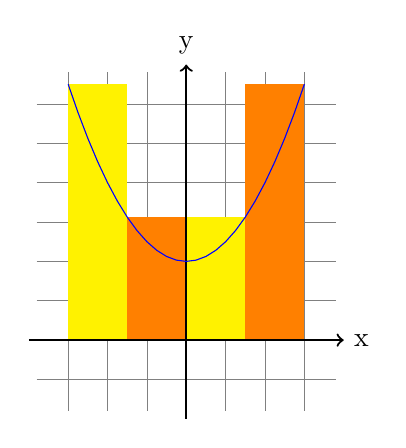
\begin{tikzpicture}
		\draw[very thin, gray, step = 0.5] (-1.9,-0.9) grid (1.9,3.4);
		\fill[yellow](-1.5,0) rectangle (-0.75,3.25);
		\fill[orange](-0.75,0) rectangle (0,1.56);
		\fill[yellow](0,0) rectangle (0.75, 1.56);
		\fill[orange](0.75,0) rectangle (1.5,3.25);
		\draw[->,thick, black](-2,0) -- (2,0) node[right]{x};
		\draw[->,thick, black](0,-1) -- (0,3.5) node[above]{y};
		\draw[blue, domain = -1.5 :1.5]  
			plot(\x, \x * \x + 1);
	\end{tikzpicture}
	\caption{oberes Riemann-Integral}
	\label{fig_int_riemann}
\end{figure}
	\textbf{Bemerkungen}
	\begin{itemize}
		\item Da $f$ beschränkt ist, gibt es $m \leq M$ in $\mathbb{R}$ mit:
		\begin{align*}
			m \leq f(x) \leq M \text{ }(x \in [a,b])
		\end{align*}
		Damit gilt für jede jede Partition $P$: 
		\begin{align*}
			m \cdot (b-a) \leq s(P,f) \leq S(P,f) \leq M \cdot (b-a)
		\end{align*}
		Ergo: $\overline{\int_a^b} f \dd{x} , \underline{\int_a^b} f \dd{x}$ 
		sind wohldefiniert.
		\item im gesamten Kapitel~\ref{kap_riemann_integral}
		werden wir Funktionen stets als 
		beschränkt annehmen
	\end{itemize}
	
}\end{Definition}

\begin{Definition}{
	Seien $P_1, P_2$ zwei Partitionen eines Intervalls. Dann heißt $P_1$ 
	\underline{Verfeinerung} von $P_2$, wenn gilt: $P_2 \subseteq P_1$ \\
	Weiterhin nennen wir $P_1 \cup P_2$ die \underline{gemeinsame} Verfeinerung 
	von $P_1$ und $P_2$
}\end{Definition}

\begin{Satz}{\label{kap09_satz16}
	Ist $P'$ eine Verfeinerung der Partition $P$ von $[a,b]$, dann gilt:
	\begin{align*}
		S (P,f) \geq & S (P',f) \\
		s(P,f) \leq & s(P',f)
	\end{align*}
	(wobei $f$ wie in Definition~\ref{def_riemann-integrierbar}
	sei) \\
	\textbf{Beweis:} Wir zeigen nur die obere Ungleichung, die andere folgt analog. 
	Wir nehmen zunächst an, dass $P'$ sich von $P$ in nur einem Element $x'$ 
	unterscheidet. Das heißt: $P' = P \cup \{x'\}$ \\
	Dann gibt es ein $i \in \mathbb{N}$ mit $x' \in [x_{i-1}, x_i]$ \newline
	(wobei $P = \{x_0, x_1, \hdots, x_{i-1}, x_i, \hdots, x_n \}$ sei).\\
	Wir definieren:
	\begin{align*}
		W_1 := & \sup_{[x_{i-1}, x']} f(x) \\
		W_2 := & sup_{[x', x_i]} f(x)
	\end{align*}
	Dann gilt: 
	\begin{align*}
		S(P,f) - S(P',f) = &M_i \Delta x_i - W_1\cdot (x' - x_{i-1}) - 
		W_2\cdot (x_i - x') \\
		= & (M_i -W_1) \cdot (x' - x_{i-1}) 
		+ (M_i - W_2)\cdot(x_i - x') \geq 0
	\end{align*}
	 Enthält von $P'$ $k$ Punkte, die nicht in $P$ enthalten sind, so führen wir 
	 obiges Verfahren insgesamt $k$-mal durch. 
	
}\end{Satz}

\begin{Satz}{\label{kap09_satz17}
	Sei $f: [a,b] \rightarrow \mathbb{R}$ beschränkt. Dann gilt:
	\begin{align*}
		\obint a b f \geq \unint{a}{b} f
	\end{align*}
	\textbf{Beweis:} Seien $P_1, P_2$ zwei Partitionierungen von $[a,b]$ und 
	$P'$ die gemeinsame Verfeinerung. Dann gilt:
	\begin{align*}
		s(P_1,f) \leq s(P',f) \leq S(P',f) \leq S(P_2, f) 
	\end{align*}
	Mit anderen Worten:
	\begin{align*}
		s(P_1, f) \leq S(P_2, f)
	\end{align*}
	für alle Partitionierungen $P_1, P_2$. \\
	Sprich: $S(P_2,f)$ ist stets obere Schranke von $s(P,f)$ für alle Partitionen 
	$P$ von $[a,b]$. Ergo:
	\begin{align*}
		\sup s(P,f) \leq S (P_2, f)
	\end{align*}
	Damit ist also $\sup s(P,f)$ untere Schranke von $S(P,f)$ ($P$ beliebige 
	Partition). \\
	Ergo: $\sup s(P,f) \leq \inf S (P,f)$  \\
	Wir haben also gezeigt:
	\begin{align*}
		\int_{\underline{a}}^b f \dd{x} = \sup s(P,f) \leq 
		\inf S(P,f) = \inf \obint ab f 
	\end{align*}
}\end{Satz}